\section{Phase 2: Translating the Decorated CPN Model to a CFG}
\label{sec:dcpntocfg}
The main purpose of this phase is to extract the control flow from the decorated CPN model and make it explicit in a control flow graph (CFG). This phase also identifies common program constructs, e.g., processes, variable, and access to variables. Furthermore, the phase finds synchronisation points, i.e., messages passing between processes. The CFG we use is a directed graph in which arcs correspond to control flow and nodes corresponds to a sequence of statements to be executed.

\subsection{Performing the Translation}
\label{sec:cpntranslation}
Given the decorated CPN model belonging to the class ProPCPN, this phase translates it into a CFG. With the decorated CPN model it is straightforward to operate on a model from a process partition perspective, e.g., to iterate through all process places in a given process partition. A CFG is constructed for all process partition in the model, thus in the producer-consumer system two CFGs are generated: one for the \code{producer} process partition and one for the \code{consumer} process partition. In Fig.~\ref{fig:prodconscfg} we see the translated CFG for the \code{producer} process partition. Below we explain how it is obtained from the decorated ProPCPN model.

\begin{figure}[b!]
\centering
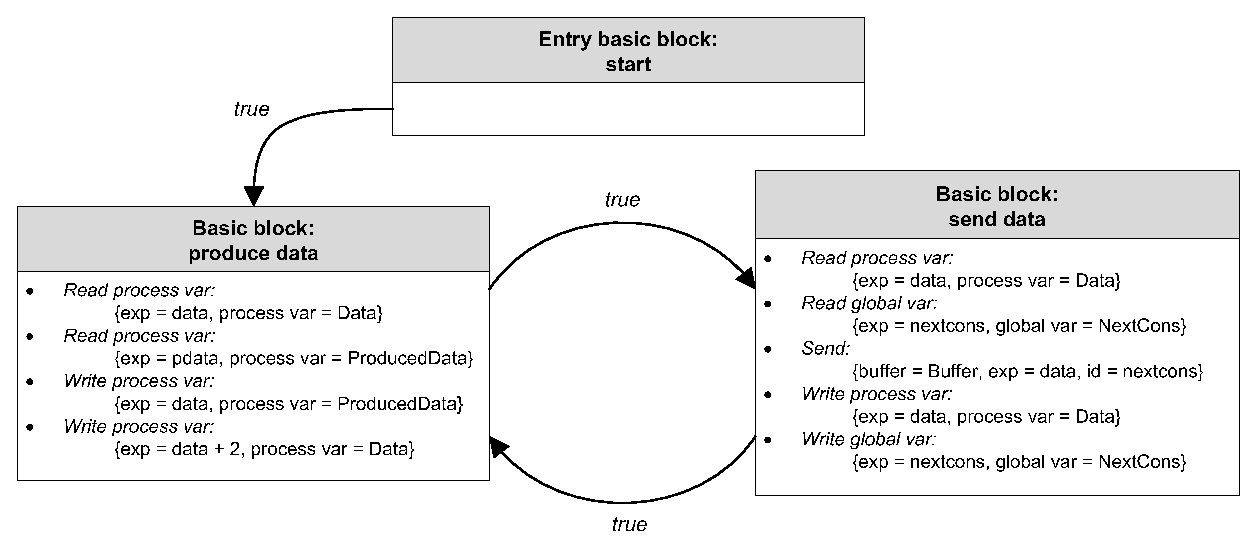
\includegraphics[width=\textwidth]{translation/dcpn_to_cfg/graphics/producerconsumercfg.eps}
\caption{The CFG of the producer process}
\label{fig:prodconscfg}
\end{figure}

%The initial state of each process instance is extracted form the initial marking of the process partition. This information is carried along in the variables for each process partition in the CFG.  \fxnote{maybe move this to another place?}

\subsubsection{Local Places}
In the CPN model, process instances use local places to store data. In a programming language this corresponds to reading/writing a variable, thus a local place is translated into a CFG \emph{process variable}. The name process variable indicates that the scope of these kinds of variables is within a given process. The \code{producer} process partition contains the two process variables \code{Data} and \code{ProducedData} corresponding to the two local places \figitem{ProducedData} and \figitem{Data} in the CPN model. 

Since a local place has an initial marking it is important to carry along this information in the corresponding process variable. The initial expressions for the variables are extracted from the initial markings of the local places. In the producer-consumer system the initial marking of the local place \figitem{ProducedData} is empty, thus the initial expression of the corresponding process variable contains the empty expression. The CFG variable node \code{Data} contains two initial expressions for the two \code{producer} process instances. In general, a process variable contains an initial expression for each process instance. 


\subsubsection{Buffer Places}
In a ProPCPN model, process instances use buffer places to share data with a particular process instance. In a programming language this corresponds to sending to and receiving from a buffer, thus a buffer place is translated into a \emph{buffer} in the CFG. In the producer-consumer system there is one buffer corresponding to the buffer place \figitem{Buffer}.


\subsubsection{Shared Places}
Process instances use shared places in the CPN model to share data with multiple process instances. In a programming language this corresponds to a global variable or some shared memory where process instances can share data. Shared places are therefore translated into \emph{global} variables in the CFG. In the producer-consumer system there is one global variable corresponding to the shared place \figitem{NextConsumer}. The initial marking of the shared place is extracted and carried along in the global variable. 

\subsubsection{Transitions}
Transitions in the CPN model are translated into \emph{basic blocks} in the CFG. In the producer process partition (see Fig. \ref{fig:prodconscfg}) the transition \figitem{ProduceData} is translated into the basic block \code{produce data} and the transition \figitem{SendData} is translated in the basic block \code{send data}. An item in a basic block in Fig.~\ref{fig:prodconscfg} should be read as follows: the name of the statement is written in italic, and the body of the statement is written in curly brackets. 

The basic block is constructed from the input and output arcs to and from the transition. Arcs are translated depending on the type of the arc. In the decorated CPN model, the connected arcs are labelled with types. In the following we consider arcs connecting transitions to local places, shared places, and buffer places.

\paragraph*{Arcs connecting a transition to a local place.}
An input arc with a arc expression on the form \code{(pid, var)} from a local place to a transition corresponds to process instance \code{pid} reading a variable \code{var}. Consider the input arc expression \code{(prod, data)} from the local place \figitem{Data} to the transition \figitem{ProduceData}. This arc is translated to a \emph{Read process var} with the expression \code{data} as shown in Fig.~\ref{fig:prodconscfg}. The \emph{Read process var} also has a pointer to the process variable \code{Data} since this is where it gets its input from.

An output arc expression on the form \code{(pid, exp)} from a transition going to a local place corresponds to process instance \code{pid} writing an \code{exp} to a variable \code{var}. Consider the output arc expression on the arc from the transition \figitem{ProduceData} to the local place \figitem{ProducedData}. This is translated to a \emph{Write process var} (seen in Fig.~\ref{fig:prodconscfg}) containing the expression \code{data} which is extracted from the CPN model. The \emph{Write process var} has a pointer to the variable \code{ProducedData} since this is where the value should be written to.

\paragraph*{Arcs connecting a transition to a buffer place.}
An input arc with the arc expression \code{(pid, var)} from a buffer place to a transition corresponds to a process receiving a message which is put into a variable \code{var}. This kind of input arc can be found in the consumer part of the producer-consumer system on the input arc (with the expression \code{(cons, data)}) from the buffer place \figitem{Buffer} to the transition \figitem{ReceiveData}. This is translated into a \emph{receive} which has the expression \code{data} meaning that the value of the received data should be read into the variable \code{data} for later use. 

An output arc with the arc expression on the form \code{(pid, exp)} from a transition to a buffer place corresponds to sending an expression \code{exp} to a process instance \code{pid}. Consider the output arc expression \code{(nextcons, data)} from the transition \figitem{SendData} to the buffer place \figitem{Buffer}. As seen in Fig.~\ref{fig:prodconscfg} this is translated a \emph{send} which points to the CFG \emph{buffer}. It contains the expression \code{data} and the receiver process instance \code{nextcons}.

\paragraph*{Arcs connecting a transition to a shared place.}
An input arc with the arc expression \code{var} from a shared place to a transition corresponds to a process reading a variable with a global scope, i.e., a variable that can be accessed and modified by multiple process instances. 

In the producer-consumer system there is a input arc expression \code{nextcons} to the transition \figitem{SendData} from the shared place \figitem{NextConsumer}. As seen in Fig.~\ref{fig:prodconscfg} this is translated to a \emph{Read global var} which points to the global variable \code{NextConsumer} and contains the expression \code{nextcons}. 

An output arc with the arc expression \code{var} from a transition to a shared place corresponds to a process writing to a global variable. Consider the output arc expression to the transition \figitem{SendData} from the shared place \figitem{NextConsumer}. This is translated to a \emph{Write global var} which points to the global variable \code{NextConsumer} and contains the expression \code{nextcons}.

\subsubsection{Process Places}
Process places in the CPN model are not explicitly translated into nodes in the CFG, but instead represented as edges between basic blocks. The idea is, for each basic block, to have a set of reachable basic blocks. In Fig.~\ref{fig:prodconscfg} we see that the basic block \code{produce data} has an edge to \code{send data} which means that after executing \code{produce data} the control should flow to the basic block \code{send data}. The condition \code{true} on the edge indicates that it is an unconditional flow of control. There is a special \emph{entry} basic block for each CFG that represent the starting point of the program. In Fig.~\ref{fig:prodconscfg} it points to the basic block \code{produce data}. In section \ref{sec:advancedissues} we explain how conditional flows are handled.

\subsection{The Structure of the Control Flow Graph}
\label{sec:cfgebnf}
A CFG is created for each process in the program, e.g., one CFG for the \code{producer} process and one for the \code{consumer} process. The CFG is a directed graph where the nodes in the graph are connected by labelled edges. The nodes in the graph represent the basic blocks and the edges represent the control flow between the blocks. The labels on the edges are \emph{conditions}, i.e., a list of boolean expressions, specifying whether the control flow can follow this edge or not.

The CFG contains a special entry basic block which is always the starting point for the control flow. The entry basic block only has outgoing edges because the control is never supposed to return to the entry point. 

The basic blocks in the CFG contains a collection of statements, e.g., read, write, send, and receive statements. Taking a closer look at, e.g. read statements, we can see that they contain a pointer to a process variable and an expression. The expression specifies a local variable that the value of the process variable is to be read into.
